\section{The Sheath Helix Model}\label{sec:sheath}
This section describes the geometry of the sheath helix and derives its corresponding boundary value field solutions. 
\subsection{Physical Development}
There are two physical interpretations for how a sheath helix is geometrically derived from a monofilar helix. Both of these interpretations begin with the tape helix of Fig. \ref{fig:tape}, where again $\delta$ represents the tape width and $p$ the turn-to-turn pitch. 
\begin{figure}[h]
	\centering
	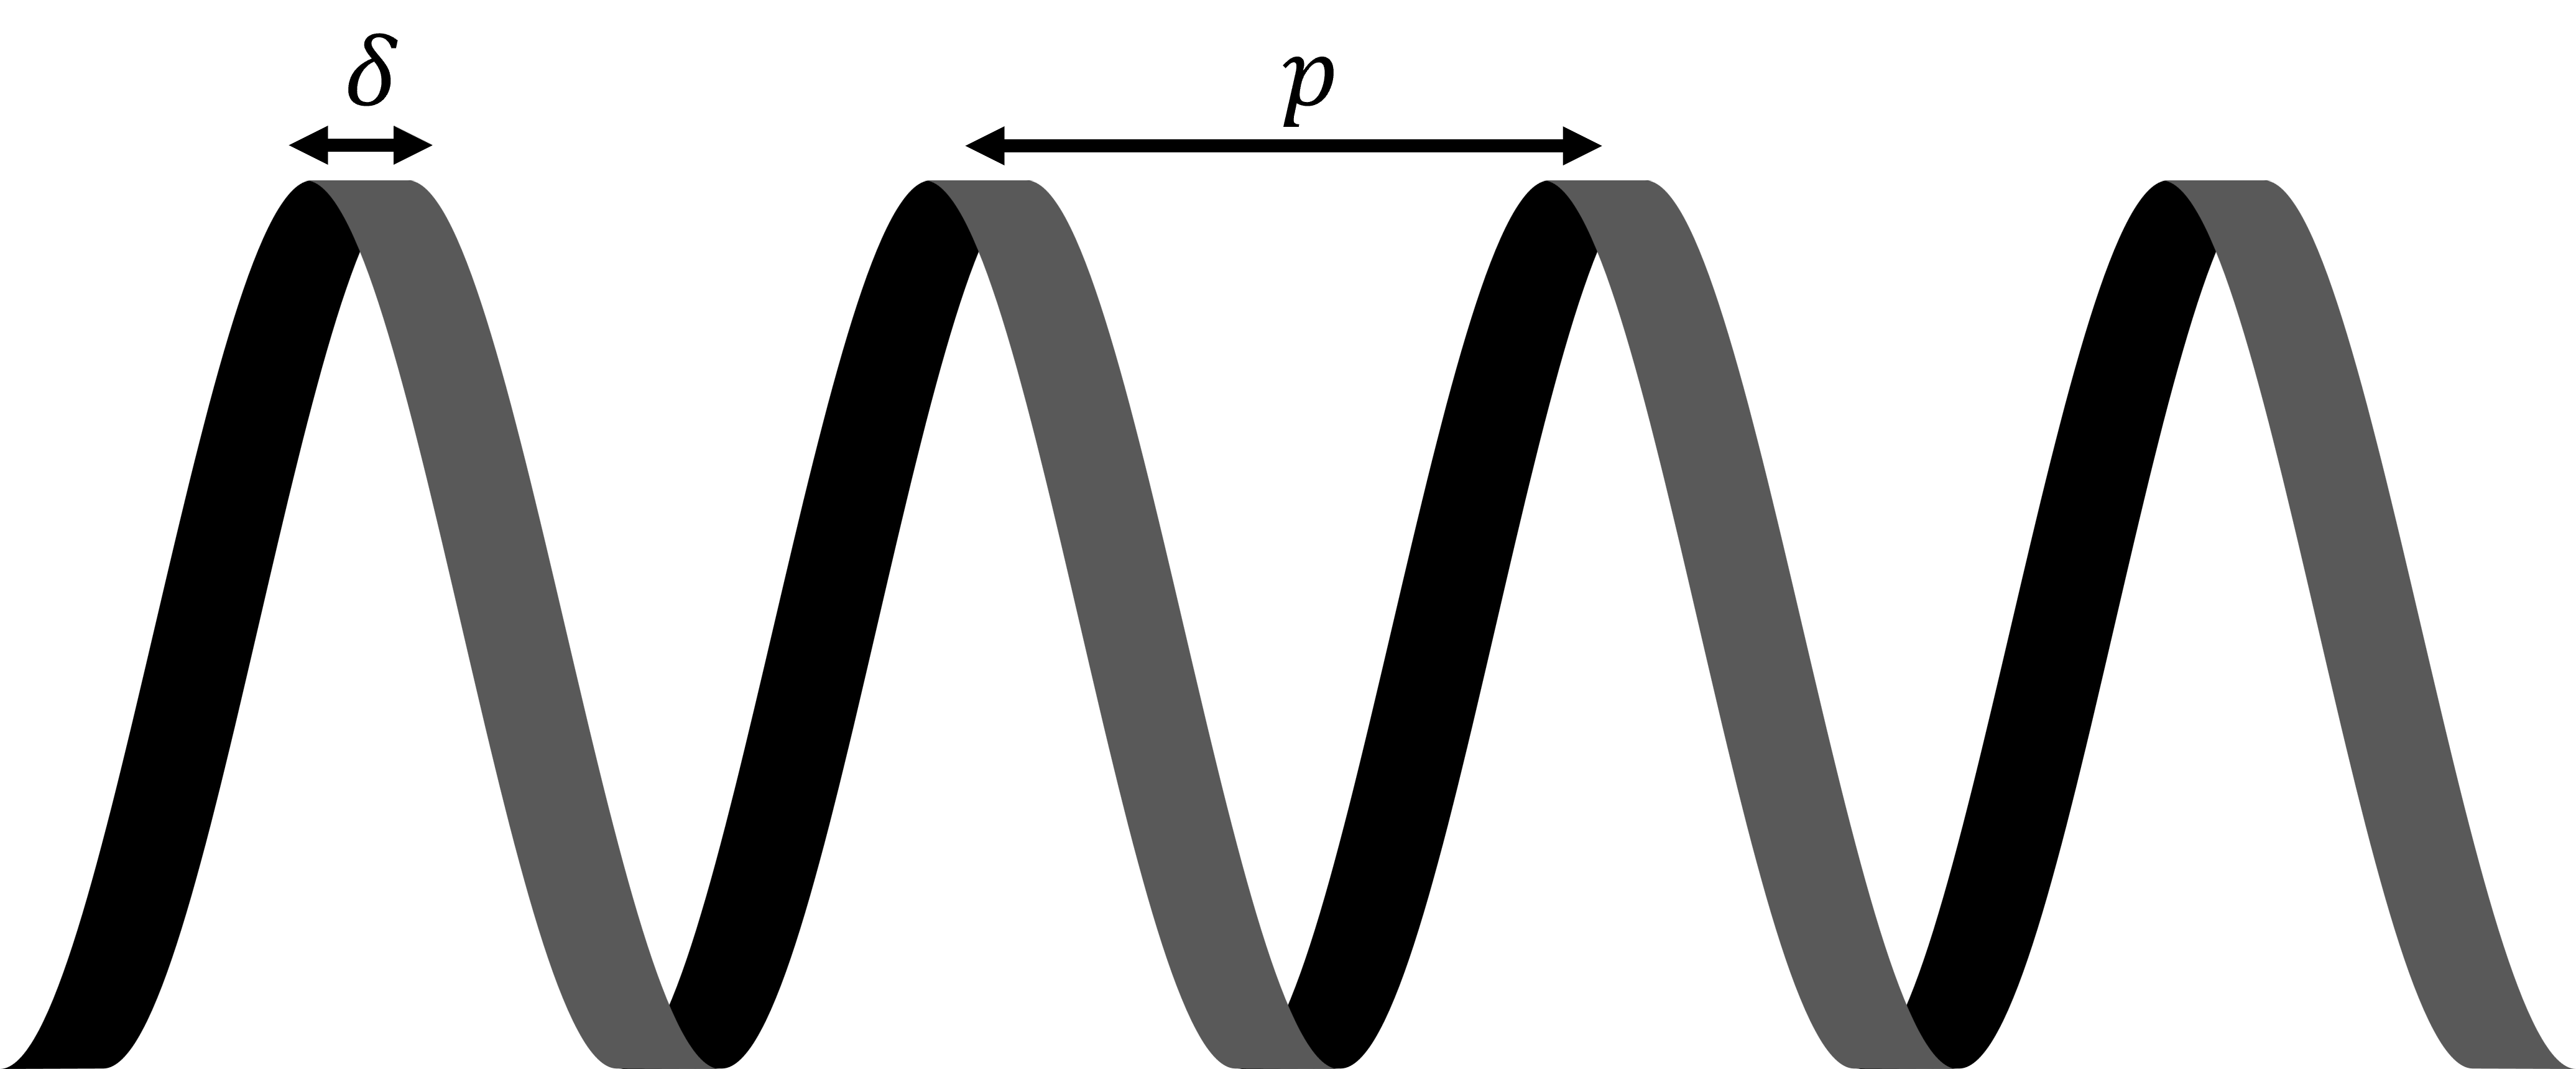
\includegraphics[width=0.6\textwidth]{tape}
	\caption{Tape helix.}
	\label{fig:tape}
\end{figure}

\hspace*{2em} \textbf{Interpretation \#1:} It is assumed that the pitch of the helix in Fig. \ref{fig:tape} is fixed. If the tape width $\delta$ is increased, the spatial gaps between adjacent turns will decrease proportionally. As $\delta \rightarrow p$, the air gaps become vanishingly small while still maintaining physical and electrical isolation from adjacent turns. In this limit, the tape helix approaches the geometry of a circular cylinder which only conducts current in the helical direction. The result is an anisotropically conducting cylindrical waveguide. 

\hspace*{2em} \textbf{Interpretation \#2:} The second interpretation for physical construction of a sheath helix is shown in Fig. \ref{fig:sheath1}. This realization assumes that additional conductors of helical tape are placed adjacent to the original -- this can equivalently be thought of as having placed axially translated copies of the original tape helix where the translation distance is equal to the width of the tape $\delta$. The tape helix conductors are all assumed to be electrically isolated from one another such that current can only flow in the helical direction. As the width of each tape helix approaches zero ($\delta\rightarrow0$) and the number of additional tape helices approaches $\infty$, the structure approaches that of an anisotropically conducting cylindrical waveguide.
\begin{figure}[h]
	\centering
	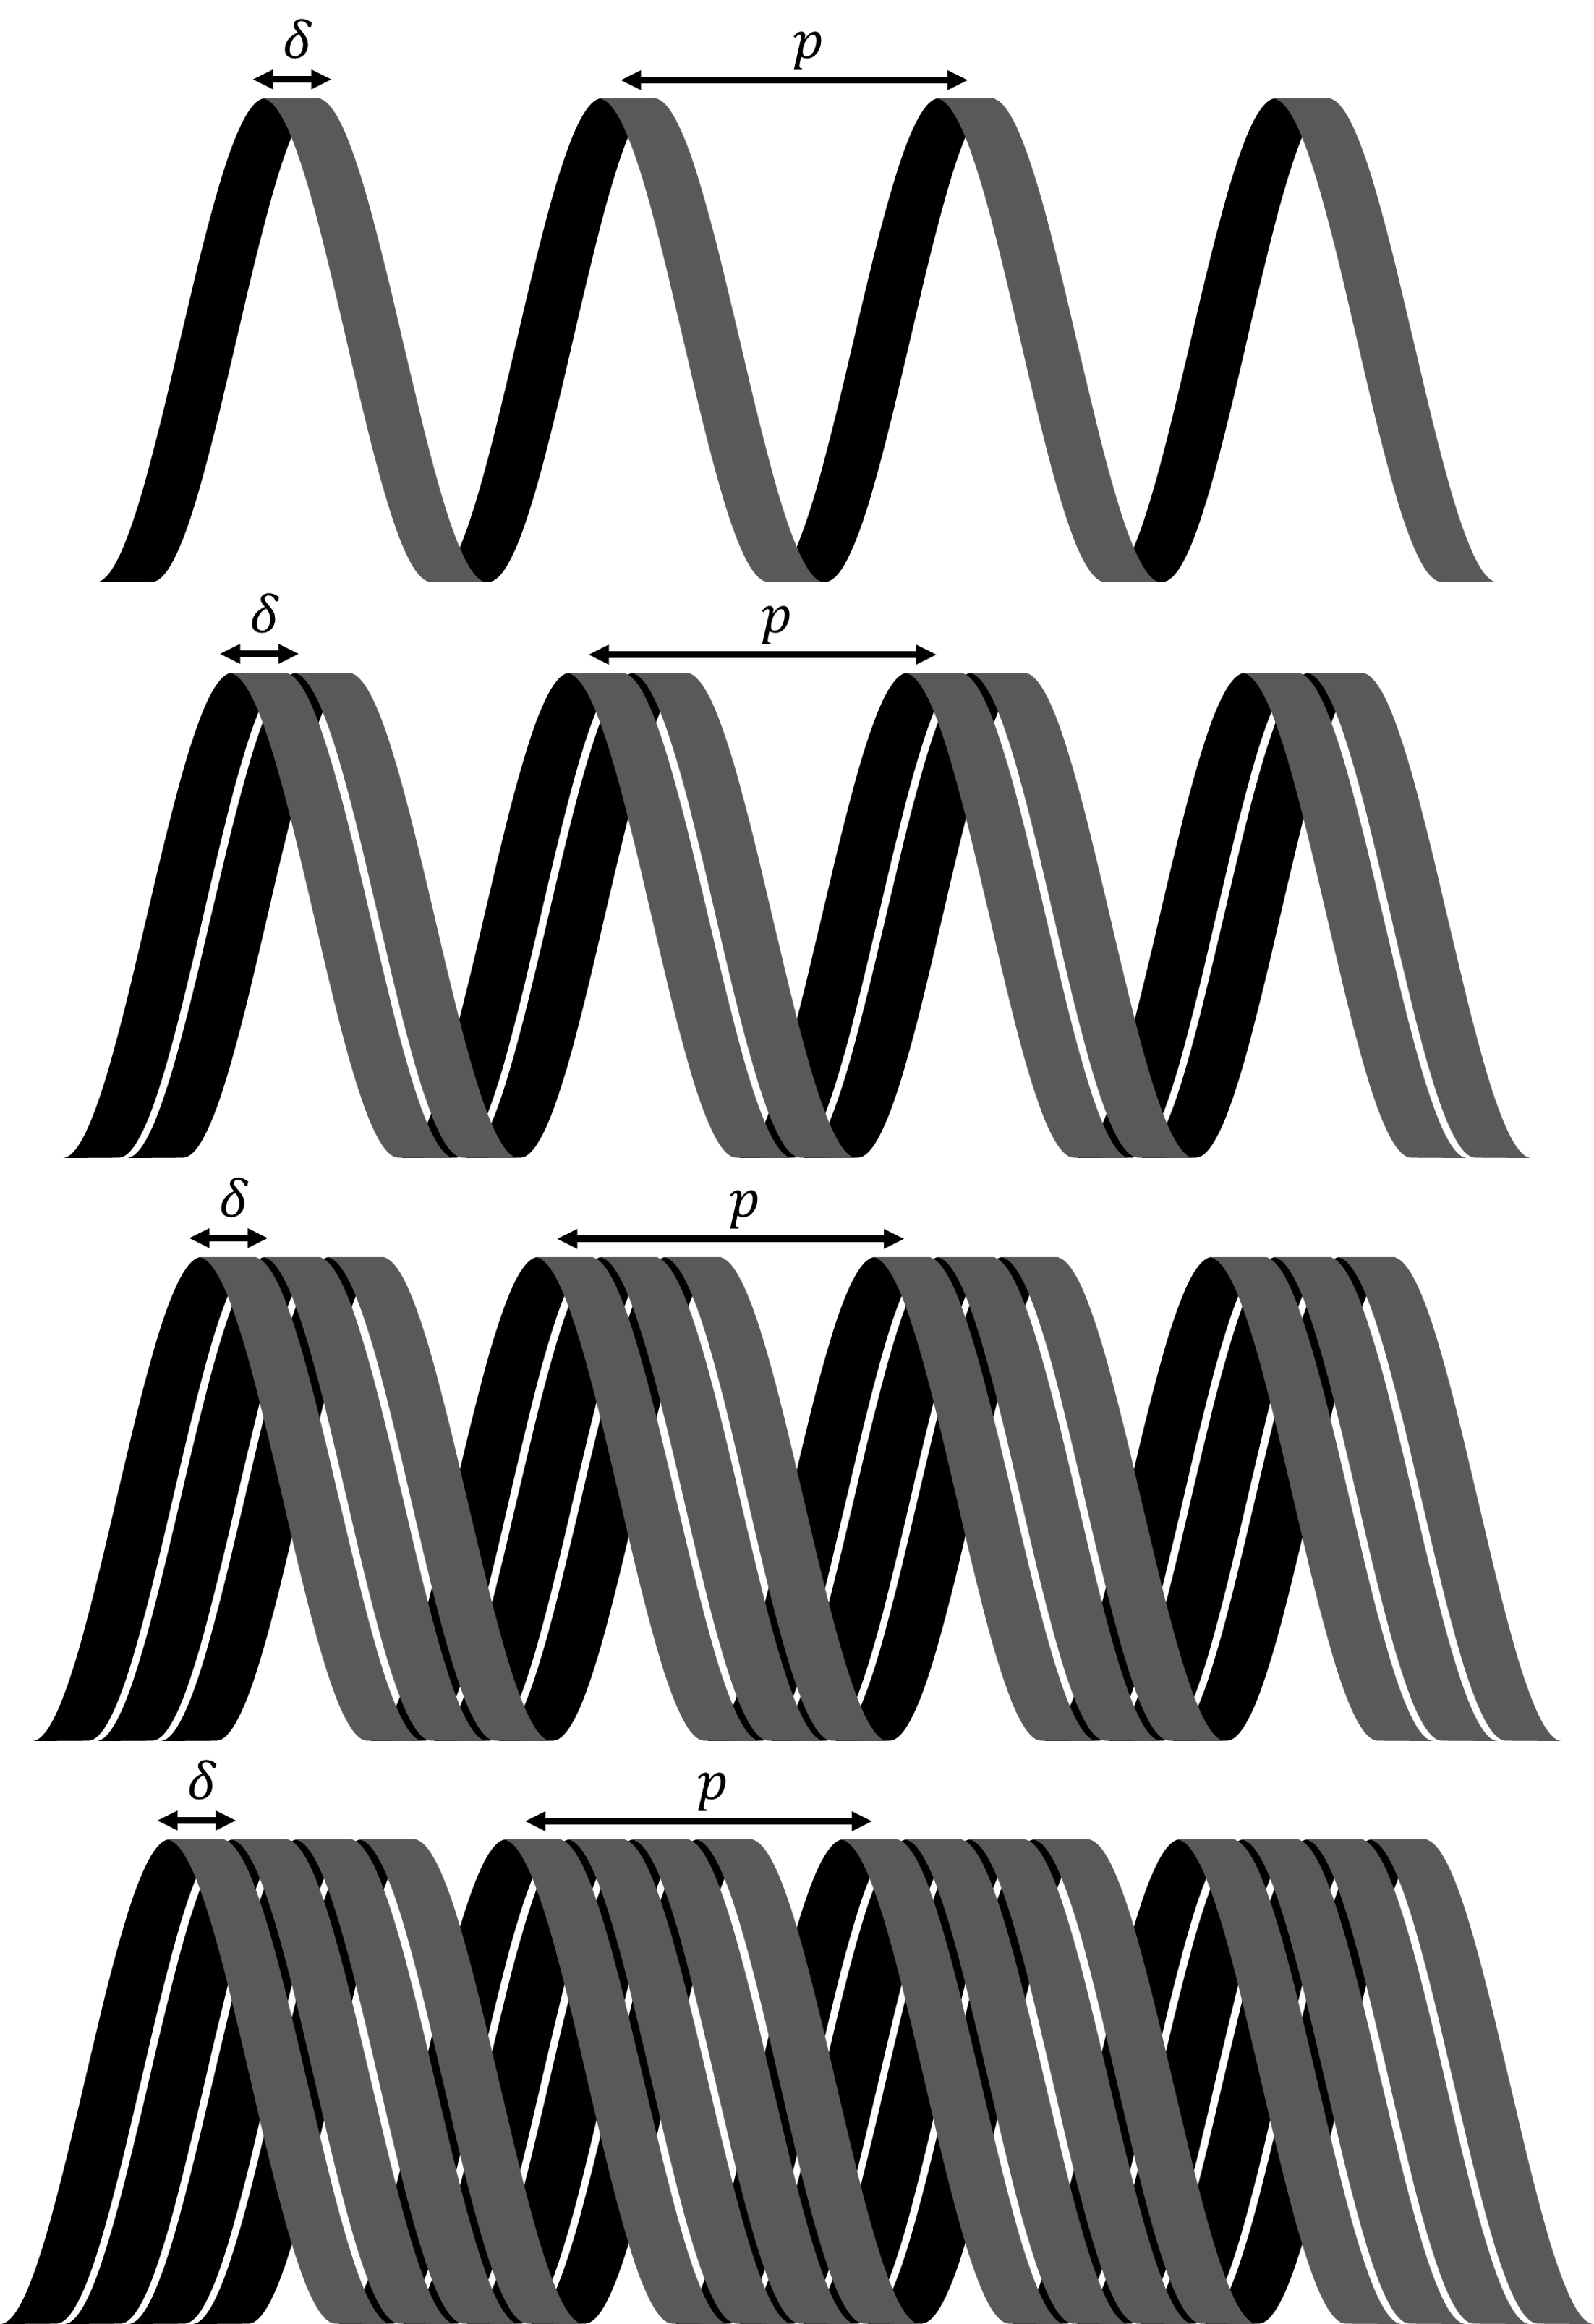
\includegraphics[width=0.6\textwidth]{sheath1}
	\caption{An equivalent sheath helix from multiple tape helices.}
	\label{fig:sheath1}
\end{figure}

It is clear from these model developments that the sheath helix should be ill-suited to model the electrical characteristics of round wire helices with large turn-to-turn pitch or tape helices with large air gaps between adjacent conductors. Conversely, the sheath helix model should remain physically approximate for helical coils with many turns per free space wavelength. 

\subsection{Field Formulation}
While not fundamental to the modeling approach, this derivation will assume that the helical coil of interest is lossless such that no attenuation is considered. The complex propagation constant is then $\gamma=j\beta$ and the fields are described by Helmholtz equations (\ref{eq:EwaveLossless})-(\ref{eq:HwaveLossless}), which are repeated below
\begin{equation}\label{eq:helmholtz1}
	\mathbf{\nabla}^2\mathbf{E} + \beta^2 \mathbf{E} = 0
\end{equation}
\begin{equation}\label{eq:helmholtz2}
	\mathbf{\nabla}^2\mathbf{H} + \beta^2 \mathbf{H} = 0
\end{equation}
where $\beta=\omega\sqrt{\mu\epsilon} = 2\pi/\lambda$ is the free space phase constant describing the spatial distribution (wavelength) of the electromagnetic waves in an unbounded medium of the same material properties. If losses are to be included in the field solution the propagation constant $\gamma$ should be adjusted accordingly. 

\subsubsection{Decomposition for Longitudinal Helmholtz Equations}\label{subsubsec:decomposition}
The equivalent anisotropically conducting helix will support a combination of TE and TM modes with traveling wave type propagation in the axial direction, resulting in axial field variations of the form $e^{j(\omega t-\beta_z z)}$. It is therefore of interest to decompose the fields into the transverse and longitudinal components. To do this, the del operator $\mathbf{\nabla}$ is itself decomposed into transverse and longitudinal components. Consider that the del operator can be written in cylindrical coordinates as
\begin{equation}\label{eq:delCyl}
	\mathbf{\nabla} = \frac{\partial}{\partial r}\hat{\mathbf{a}}_{r} + \frac{1}{r}\frac{\partial}{\partial \phi}\hat{\mathbf{a}}_{\phi} + \frac{\partial}{\partial z}\hat{\mathbf{a}}_{z}
\end{equation}
This can be split into the transverse and longitudinal components as $\nabla = \nabla_t + \nabla_l$, where 
\begin{equation}\label{eq:delT}
	\mathbf{\nabla}_t = \frac{\partial}{\partial r}\hat{\mathbf{a}}_{r} + \frac{1}{r}\frac{\partial}{\partial \phi}\hat{\mathbf{a}}_{\phi}
\end{equation}
\begin{equation}\label{eq:delL}
	\mathbf{\nabla}_l = \frac{\partial}{\partial z}\hat{\mathbf{a}}_{z}
\end{equation}
Since the axial propagation is of traveling wave form, the partial derivative can be written as $\partial / \partial z = -j\beta_z$, reducing (\ref{eq:delL}) to
\begin{equation}\label{eq:delLr}
	\mathbf{\nabla}_l = -j\beta_z\hat{\mathbf{a}}_{z}
\end{equation}
The Laplacian operator can then be found from (\ref{eq:delT}) and (\ref{eq:delLr}) as
\begin{equation}\label{eq:Laplacian}
	\begin{split}
	\mathbf{\nabla}^2 &= \nabla \cdot \nabla = (\nabla_t + \nabla_l) \cdot (\nabla_t + \nabla_l) = (\nabla_t + -j\beta_z\hat{\mathbf{a}}_{z}) \cdot (\nabla_t + -j\beta_z\hat{\mathbf{a}}_{z}) \\ 
	&= \nabla_t \cdot \nabla_t + \nabla_t \cdot -j\beta_z\hat{\mathbf{a}}_{z} + -j\beta_z\hat{\mathbf{a}}_{z} \cdot \nabla_t + -j\beta_z\hat{\mathbf{a}}_{z} \cdot -j\beta_z\hat{\mathbf{a}}_{z} \\
	&= \nabla_t^2 + j^2\beta_z^2 = \nabla_t^2 - \beta_z^2
	\end{split}
\end{equation}
Inserting the decomposed Laplacian (\ref{eq:Laplacian}) into Helmholtz equations (\ref{eq:helmholtz1}) and (\ref{eq:helmholtz2}) gives  
\begin{equation}\label{eq:helmholtz3}
	(\nabla_t^2 - \beta_z^2)\mathbf{E} + \beta^2 \mathbf{E} = \nabla_t^2\mathbf{E} + (\beta^2 - \beta_z^2)\mathbf{E} = 0
\end{equation}
\begin{equation}\label{eq:helmholtz4}
	(\nabla_t^2 - \beta_z^2)\mathbf{H} + \beta^2 \mathbf{H} = \nabla_t^2\mathbf{H} + (\beta^2 - \beta_z^2)\mathbf{H} = 0
\end{equation}
Combining (\ref{eq:helmholtz3}) and (\ref{eq:helmholtz4}) with the cylindrical constraint equation (\ref{eq:constraintCyl}) results in Helmholtz equations in transverse coordinates
\begin{equation}\label{eq:helmholtz5}
	\nabla_t^2 \mathbf{E} + \beta_r^2 \mathbf{E} = 0
\end{equation}
\begin{equation}\label{eq:helmholtz6}
	\nabla_t^2 \mathbf{H} + \beta_r^2 \mathbf{H} = 0
\end{equation}
(\ref{eq:helmholtz5}) and (\ref{eq:helmholtz6}) can be separated into their respective transverse and longitudal operations as
\begin{equation}\label{eq:helmholtz7}
	\nabla_t^2 E_t + \beta_r^2 E_t = 0
\end{equation}
\begin{equation}\label{eq:helmholtz8}
	\nabla_t^2 H_t + \beta_r^2 H_t = 0
\end{equation}
and 
\begin{equation}\label{eq:helmholtz9}
	\nabla_t^2 E_z + \beta_r^2 E_z = 0
\end{equation}
\begin{equation}\label{eq:helmholtz10}
	\nabla_t^2 H_z + \beta_r^2 H_z = 0
\end{equation}

\subsubsection{Assumption of Solutions and The Kraus $T_0$ Transmission Mode}\label{subsubsec:assumption1}
The anisotropically conducting helical waveguide will support both TE and TM electromagnetic field configurations propagating in the axial direction such that there exists an axial component of both the electric and magnetic field. The radial wavenumber $\beta_r$ describes the spatial electrical characterisitcs in the radial direction and may take two forms: (1) a fast wave structure ($\beta_z^2 \le \beta^2$) that has $\beta_r^2 \ge 0$, describing broadside radiative propagation from the sheath helix, or (2) a slow wave structure ($\beta_z^2 > \beta^2$) that has $\beta_r^2 < 0$, describing evanescent characteristics asssociated with tightly bound waves propagating along the helical structure. 

While helical coils had been studied in the context of ``low frequency" inductances and circuit elements since the late 1800's (e.g., \cite{tesla1, pocklington}), it was not until 1946 that Dr. John D. Kraus invented the first helical antenna at Ohio State University \cite{kraus2}. Since that time, Dr. Kraus has pioneered the rapid and widespread development of helical coils as antenna elements, leading to a substantial increase in the modeling capability and physical understanding of electrical characteristics of helical coils. In his classic antennas textbook \cite{kraus2}, Dr. Kraus makes the following distinction with regard to modes of operation in a helical coil:

\hspace*{2em} \textit{\textbf{The Transmission Mode:}} This mode ``describes the manner in which an electromagnetic wave is propagated along an infinite helix as though the helix constitutes an infinite transmission line or waveguide".

\hspace*{2em} \textit{\textbf{The Radiation Mode:}} This mode describes ``the general form of the far-field [radiation] pattern of a finite helical antenna".

This document is primarily interested in leveraging the sheath helix model to describe the electrical characteristics at the terminals of a helix when used as a low frequency inductance or resonator. In this context, the transmission mode is clearly that of interest and it is expected that the fields will travel as slow waves tightly coupled to the helical geometry. It is then appropriate to explicitly write the expected form of the constraint equation by taking $\beta_{r}^2 = \beta_{z}^2 - \beta^2$. The axial fields are then assumed to take the following form 
\begin{equation}\label{eq:assumedE}
	E_{z}^{i,o} = [A_{m}^{i,o}I_{m}(\beta_{r,m}r) + B_{m}^{i,o}K_{m}(\beta_{r,m}r)]e^{j(\omega t - m\phi-\beta_{z}z)}
\end{equation}
\begin{equation}\label{eq:assumedH}
	H_{z}^{i,o} = [C_{m}^{i,o}I_{m}(\beta_{r,m}r) + D_{m}^{i,o}K_{m}(\beta_{r,m}r)]e^{j(\omega t - m\phi-\beta_{z}z)}
\end{equation}
In (\ref{eq:assumedE}) and (\ref{eq:assumedH}), the superscripts $i$ and $o$ delineate the fields inside and outside the sheath helix boundary, respectively, and are separated by the perfectly conducting sheath at $r=a$. $A_m$, $B_m$, $C_m$, and $D_m$ are arbitrary constants which are to be determined from the anisotropic boundary conditions, and $m$ represents the order of the wave mode as defined by (\ref{eq:sep1cyl}) and (\ref{eq:sep1cy2}). By comparing the assumptions of the field forms to the wave functions described in Table \ref{tab:cylWaves}, it is clear that the axial field components have been assumed to have radially evanescent waves and traveling waves in the $\phi$ and $z$ direction. 

The lowest transmission mode supported by a helix, designated by Kraus as the $T_0$ mode and sometimes subsequently referred to as the `Kraus' mode, has adjacent regions of positive and negative charge along the helical conductor that are separated by many winding turns. This mode is considered appropriate when the arc length of a single winding turn is very small compared to the electrical wavelength ($L_n \ll \lambda$) and is that found on ``low frequency" inductances. It is this background that justifies neglecting azimuthal field dependence for the remainder of this document ($\partial/\partial\phi=0, m=0$), although it is emphasized here that the following derivations may also be performed for arbitrary modes $m$ that become important at higher frequencies. The field solutions (\ref{eq:assumedE}) and (\ref{eq:assumedH}) with $m=0$ reduce to
\begin{equation}\label{eq:assumedEt0}
	E_{z}^{i,o} = [A^{i,o}I_{0}(\beta_{r}r) + B^{i,o}K_{0}(\beta_{r}r)]e^{j(\omega t - \beta_{z}z)}
\end{equation}
\begin{equation}\label{eq:assumedHt0}
	H_{z}^{i,o} = [C^{i,o}I_{0}(\beta_{r}r) + D^{i,o}K_{0}(\beta_{r}r)]e^{j(\omega t - \beta_{z}z)}
\end{equation}


\subsubsection{Determination of Coefficients Through Asymptotic Behavior}\label{subsubsec:asymptotic}
In order to determine the coefficients $A^{i,o}$, $B^{i,o}$, $C^{i,o}$, and $D^{i,o}$, it is necessary to enforce the boundary conditions of the problem. However, by combining intuitive asymptotic behavior of the fields with the known asymptotic behavior of the modified Bessel functions of first and second kind and order 0, vanishing constants may be inferred. For example, inside the sheath helix the fields must be everywhere finite   and outside the sheath helix the fields must vanish as $r\rightarrow\infty$. To satisfy these conditions, the asymptotic behavior of $I_o(r)$ and $K_o(r)$, shown in Fig. \ref{fig:bessel}, clearly requires $A^o=C^o=B^i=D^i=0$. The axial field components then reduce to 
\begin{equation}\label{eq:Ezi}
	E_{z}^{i} = A^{i}I_{0}(\beta_{r}r)e^{j(\omega t - \beta_{z}z)}
\end{equation}
\begin{equation}\label{eq:Hzi}
	H_{z}^{i} = C^{i}I_{0}(\beta_{r}r)e^{j(\omega t - \beta_{z}z)}
\end{equation}
\begin{equation}\label{eq:Ezo}
	E_{z}^{o} = B^{o}K_{0}(\beta_{r}r)e^{j(\omega t - \beta_{z}z)}
\end{equation}
\begin{equation}\label{eq:Hzo}
	H_{z}^{o} = D^{o}K_{0}(\beta_{r}r)e^{j(\omega t - \beta_{z}z)}
\end{equation}
\subsection{Field Solutions}
Having determined the final form of the axial field components (\ref{eq:Ezi})-(\ref{eq:Hzo}) both inside and outside the sheath helix, the remaining field solutions must be determined. This is done by applying Maxwell's equations in cylindrical coordinates. 
\subsubsection{Maxwell's Equations in Cylindrical Coordinates}
Ampere's Law and Faraday's Law in a source-free and lossless medium can be written in differential form as
\begin{equation}\label{eq:ampere}
	\nabla \times \mathbf{H} = \epsilon \frac{\partial \mathbf{E}}{\partial t}
\end{equation}
\begin{equation}\label{eq:faraday}
	\nabla \times \mathbf{E} = - \mu \frac{\partial \mathbf{H}}{\partial t}
\end{equation}
The curl of a vector field in cylindrical coordinates is found as
\begin{equation}\label{eq:curl}
	\begin{split}
		\nabla \times \mathbf{A} &= \frac{1}{r}
		\begin{vmatrix}
			\hat{\mathbf{a}}_r & \hat{\mathbf{a}}_\phi r & \hat{\mathbf{a}}_z \\
			\frac{\partial}{\partial r} & \frac{\partial}{\partial \phi} & \frac{\partial}{\partial z} \\
			A_r & r A_\phi & A_z
		\end{vmatrix}
		\\
		=
		\hat{\mathbf{a}}_r \left( \frac{1}{r} \frac{\partial A_z}{\partial \phi} - \frac{\partial A_\phi}{\partial z} \right)
		+ &\hat{\mathbf{a}}_\phi \left( \frac{\partial A_r}{\partial z} - \frac{\partial A_z}{\partial r} \right)
		+ \hat{\mathbf{a}}_z \frac{1}{r} \left( \frac{\partial}{\partial r}(r A_\phi) - \frac{\partial A_r}{\partial \phi} \right)
	\end{split}
\end{equation}
Ampere's Law and Faraday's Law then result in 
\begin{equation}\label{eq:ampere1}
	\begin{split}
	&\hat{\mathbf{a}}_r \left( \frac{1}{r} \frac{\partial H_z}{\partial \phi} - \frac{\partial H_\phi}{\partial z} \right)
	+ \hat{\mathbf{a}}_\phi \left( \frac{\partial H_r}{\partial z} - \frac{\partial H_z}{\partial r} \right)
	+ \hat{\mathbf{a}}_z \frac{1}{r} \left( \frac{\partial}{\partial r}(r H_\phi) - \frac{\partial H_r}{\partial \phi} \right) \\
	=
	&\hat{\mathbf{a}}_r \varepsilon \frac{\partial E_r}{\partial t}
	+ \hat{\mathbf{a}}_\phi \varepsilon \frac{\partial E_\phi}{\partial t}
	+ \hat{\mathbf{a}}_z \varepsilon \frac{\partial E_z}{\partial t}
	\end{split}
\end{equation}
\begin{equation}\label{eq:faraday1}
	\begin{split}
	&\hat{\mathbf{a}}_r \left( \frac{1}{r} \frac{\partial E_z}{\partial \phi} - \frac{\partial E_\phi}{\partial z} \right)
	+ \hat{\mathbf{a}}_\phi \left( \frac{\partial E_r}{\partial z} - \frac{\partial E_z}{\partial r} \right)
	+ \hat{\mathbf{a}}_z \frac{1}{r} \left( \frac{\partial}{\partial r}(r E_\phi) - \frac{\partial E_r}{\partial \phi} \right) \\
	=
	- &\hat{\mathbf{a}}_r \mu \frac{\partial H_r}{\partial t}
	- \hat{\mathbf{a}}_\phi \mu \frac{\partial H_\phi}{\partial t}
	- \hat{\mathbf{a}}_z \mu \frac{\partial H_z}{\partial t}
	\end{split}
\end{equation}
(\ref{eq:ampere1}) and (\ref{eq:faraday1}) result in the following relationships
\begin{equation}\label{eq:reln1}
	\frac{1}{r} \frac{\partial H_z}{\partial \phi} - \frac{\partial H_\phi}{\partial z} = \varepsilon \frac{\partial E_r}{\partial t}
\end{equation}
\begin{equation}\label{eq:reln2}
	\frac{\partial H_r}{\partial z} - \frac{\partial H_z}{\partial r} = \varepsilon \frac{\partial E_\phi}{\partial t}
\end{equation}
\begin{equation}\label{eq:reln3}
	\frac{1}{r} \left( \frac{\partial}{\partial r} (r H_\phi) - \frac{\partial H_r}{\partial \phi} \right) = \varepsilon \frac{\partial E_z}{\partial t}
\end{equation}
\begin{equation}\label{eq:reln4}
	\frac{1}{r} \frac{\partial E_z}{\partial \phi} - \frac{\partial E_\phi}{\partial z} = -\mu \frac{\partial H_r}{\partial t}
\end{equation}
\begin{equation}\label{eq:reln5}
	\frac{\partial E_r}{\partial z} - \frac{\partial E_z}{\partial r} = -\mu \frac{\partial H_\phi}{\partial t}
\end{equation}
\begin{equation}\label{eq:reln6}
	\frac{1}{r} \left( \frac{\partial}{\partial r} (r E_\phi) - \frac{\partial E_r}{\partial \phi} \right) = -\mu \frac{\partial H_z}{\partial t}
\end{equation}
Recalling the assumption of azimuthal symmetry ($\partial/\partial \phi = 0$), (\ref{eq:reln1})-(\ref{eq:reln6}) reduce to  
\begin{equation}\label{eq:reln7}
	- \frac{\partial H_\phi}{\partial z} = \varepsilon \frac{\partial E_r}{\partial t}
\end{equation}
\begin{equation}\label{eq:reln8}
	\frac{\partial H_r}{\partial z} - \frac{\partial H_z}{\partial r} = \varepsilon \frac{\partial E_\phi}{\partial t}
\end{equation}
\begin{equation}\label{eq:reln9}
	\frac{1}{r} \frac{\partial}{\partial r} r H_\phi = \varepsilon \frac{\partial E_z}{\partial t}
\end{equation}
\begin{equation}\label{eq:reln10}
	- \frac{\partial E_\phi}{\partial z} = -\mu \frac{\partial H_r}{\partial t}
\end{equation}
\begin{equation}\label{eq:reln11}
	\frac{\partial E_r}{\partial z} - \frac{\partial E_z}{\partial r} = -\mu \frac{\partial H_\phi}{\partial t}
\end{equation}
\begin{equation}\label{eq:reln12}
	\frac{1}{r} \frac{\partial}{\partial r} r E_\phi = -\mu \frac{\partial H_z}{\partial t}
\end{equation}

\subsubsection{The Transverse Fields}\label{subsubsec:transverse}
The partial time derivatives of the axial field components are found as
\begin{equation}
	\frac{\partial E_z^i}{\partial t} = \frac{\partial}{\partial t} A^i I_0(\beta_r r) e^{j(\omega t - \beta_z z)} = j\omega A^i I_0(\beta_r r) e^{j(\omega t - \beta_z z)}
	\label{eq:Ez_i}
\end{equation}
\begin{equation}
	\frac{\partial H_z^i}{\partial t} = \frac{\partial}{\partial t} C^i I_0(\beta_r r) e^{j(\omega t - \beta_z z)} = j\omega C^i I_0(\beta_r r) e^{j(\omega t - \beta_z z)}
	\label{eq:Hz_i}
\end{equation}
\begin{equation}
	\frac{\partial E_z^o}{\partial t} = \frac{\partial}{\partial t} B^o K_0(\beta_r r) e^{j(\omega t - \beta_z z)} = j\omega B^o K_0(\beta_r r) e^{j(\omega t - \beta_z z)}
	\label{eq:Ez_o}
\end{equation}
\begin{equation}
	\frac{\partial H_z^o}{\partial t} = \frac{\partial}{\partial t} D^o K_0(\beta_r r) e^{j(\omega t - \beta_z z)} = j\omega D^o K_0(\beta_r r) e^{j(\omega t - \beta_z z)}
	\label{eq:Hz_o}
\end{equation}
Plugging (\ref{eq:Ez_i})-(\ref{eq:Hz_o}) into (\ref{eq:reln9}) and (\ref{eq:reln12}) and enforcing the identities of Bessel functions $\int rI_{0}(bx)=r/b\cdot I_{1}(bx)$ and $\int rK_{0}(bx)=r/b\cdot K_{1}(bx)$, the azimuthal field components are found as
\begin{equation}
	\begin{split}
		\frac{1}{r} \frac{\partial}{\partial r}(r H_\phi^i) &= \varepsilon \frac{\partial E_z^i}{\partial t} \\
		&= j \omega \varepsilon A^i I_0(\beta_r r) e^{j(\omega t - \beta_z z)} \\
		\Rightarrow \frac{\partial}{\partial r}(r H_\phi^i) &= j \omega \varepsilon r A^i I_0(\beta_r r) e^{j(\omega t - \beta_z z)} \\
		\Rightarrow r H_\phi^i &= \int j \omega \varepsilon r A^i I_0(\beta_r r) e^{j(\omega t - \beta_z z)} \, dr \\
		&= j \omega \varepsilon A^i e^{j(\omega t - \beta_z z)} \int r I_0(\beta_r r) \, dr \\
		&= j \omega \varepsilon A^i e^{j(\omega t - \beta_z z)} \cdot \frac{r}{\beta_r} I_1(\beta_r r) \\
		\Rightarrow H_\phi^i &= \frac{j \omega \varepsilon}{\beta_r} A^i I_1(\beta_r r) e^{j(\omega t - \beta_z z)}
	\end{split}
	\label{eq:Hphi_i}
\end{equation}

\begin{equation}
	\begin{split}
		\frac{1}{r} \frac{\partial}{\partial r}(r E_\phi^i) &= -\mu \frac{\partial H_z^i}{\partial t} \\
		&= -j \omega \mu C^i I_0(\beta_r r) e^{j(\omega t - \beta_z z)} \\
		\Rightarrow \frac{\partial}{\partial r}(r E_\phi^i) &= -j \omega \mu r C^i I_0(\beta_r r) e^{j(\omega t - \beta_z z)} \\
		\Rightarrow r E_\phi^i &= \int -j \omega \mu r C^i I_0(\beta_r r) e^{j(\omega t - \beta_z z)} \, dr \\
		&= -j \omega \mu C^i e^{j(\omega t - \beta_z z)} \int r I_0(\beta_r r) \, dr \\
		&= -j \omega \mu C^i e^{j(\omega t - \beta_z z)} \cdot \frac{r}{\beta_r} I_1(\beta_r r) \\
		\Rightarrow E_\phi^i &= -\frac{j \omega \mu}{\beta_r} C^i I_1(\beta_r r) e^{j(\omega t - \beta_z z)}
	\end{split}
	\label{eq:Ephi_i}
\end{equation}

\begin{equation}
	\begin{split}
		\frac{1}{r} \frac{\partial}{\partial r}(r H_\phi^o) &= \varepsilon \frac{\partial E_z^o}{\partial t} \\
		&= j \omega \varepsilon B^o K_0(\beta_r r) e^{j(\omega t - \beta_z z)} \\
		\Rightarrow \frac{\partial}{\partial r}(r H_\phi^o) &= j \omega \varepsilon r B^o K_0(\beta_r r) e^{j(\omega t - \beta_z z)} \\
		\Rightarrow r H_\phi^o &= \int j \omega \varepsilon r B^o K_0(\beta_r r) e^{j(\omega t - \beta_z z)} \, dr \\
		&= j \omega \varepsilon B^o e^{j(\omega t - \beta_z z)} \int r K_0(\beta_r r) \, dr \\
		&= j \omega \varepsilon B^o e^{j(\omega t - \beta_z z)} \cdot \left( -\frac{r}{\beta_r} K_1(\beta_r r) \right) \\
		\Rightarrow H_\phi^o &= -\frac{j \omega \varepsilon}{\beta_r} B^o K_1(\beta_r r) e^{j(\omega t - \beta_z z)}
	\end{split}
	\label{eq:Hphi_o}
\end{equation}

\begin{equation}
	\begin{split}
		\frac{1}{r} \frac{\partial}{\partial r}(r E_\phi^o) &= -\mu \frac{\partial H_z^o}{\partial t} \\
		&= -j \omega \mu D^o K_0(\beta_r r) e^{j(\omega t - \beta_z z)} \\
		\Rightarrow \frac{\partial}{\partial r}(r E_\phi^o) &= -j \omega \mu r D^o K_0(\beta_r r) e^{j(\omega t - \beta_z z)} \\
		\Rightarrow r E_\phi^o &= \int -j \omega \mu r D^o K_0(\beta_r r) e^{j(\omega t - \beta_z z)} \, dr \\
		&= -j \omega \mu D^o e^{j(\omega t - \beta_z z)} \int r K_0(\beta_r r) \, dr \\
		&= -j \omega \mu D^o e^{j(\omega t - \beta_z z)} \cdot \left( -\frac{r}{\beta_r} K_1(\beta_r r) \right) \\
		\Rightarrow E_\phi^o &= \frac{j \omega \mu}{\beta_r} D^o K_1(\beta_r r) e^{j(\omega t - \beta_z z)}
	\end{split}
	\label{eq:Ephi_o}
\end{equation}

The partial derivatives of the azimuthal field components with respect to the axial coordinate are then found as
\begin{equation}
	\begin{split}
		-\frac{\partial H_\phi^i}{\partial z} &= -\frac{\partial}{\partial z} \left( \frac{j \omega \varepsilon}{\beta_r} A^i I_1(\beta_r r) e^{j(\omega t - \beta_z z)} \right) = -\frac{j \omega \varepsilon}{\beta_r} A^i I_1(\beta_r r) \frac{\partial}{\partial z} \left( e^{j(\omega t - \beta_z z)} \right) \\
		&= j^2 \frac{\omega \varepsilon \beta_z}{\beta_r} A^i I_1(\beta_r r) e^{j(\omega t - \beta_z z)} = -\frac{\omega \varepsilon \beta_z}{\beta_r} A^i I_1(\beta_r r) e^{j(\omega t - \beta_z z)}
	\end{split}
	\label{eq:dHz_i}
\end{equation}
\begin{equation}
	\begin{split}
		-\frac{\partial E_\phi^i}{\partial z} &= -\frac{\partial}{\partial z} \left( -\frac{j \omega \mu}{\beta_r} C^i I_1(\beta_r r) e^{j(\omega t - \beta_z z)} \right) = \frac{j \omega \mu}{\beta_r} C^i I_1(\beta_r r) \frac{\partial}{\partial z} \left( e^{j(\omega t - \beta_z z)} \right) \\
		&= -j^2 \frac{\omega \mu \beta_z}{\beta_r} C^i I_1(\beta_r r) e^{j(\omega t - \beta_z z)} = \frac{\omega \mu \beta_z}{\beta_r} C^i I_1(\beta_r r) e^{j(\omega t - \beta_z z)}
	\end{split}
	\label{eq:dEz_i}
\end{equation}
\begin{equation}
	\begin{split}
		-\frac{\partial H_\phi^o}{\partial z} &= -\frac{\partial}{\partial z} \left( -\frac{j \omega \varepsilon}{\beta_r} B^o K_1(\beta_r r) e^{j(\omega t - \beta_z z)} \right) = \frac{j \omega \varepsilon}{\beta_r} B^o K_1(\beta_r r) \frac{\partial}{\partial z} \left( e^{j(\omega t - \beta_z z)} \right) \\
		&= -j^2 \frac{\omega \varepsilon \beta_z}{\beta_r} B^o K_1(\beta_r r) e^{j(\omega t - \beta_z z)} = \frac{\omega \varepsilon \beta_z}{\beta_r} B^o K_1(\beta_r r) e^{j(\omega t - \beta_z z)}
	\end{split}
	\label{eq:dHz_o}
\end{equation}
\begin{equation}
	\begin{split}
		-\frac{\partial E_\phi^o}{\partial z} &= -\frac{\partial}{\partial z} \left( \frac{j \omega \mu}{\beta_r} D^o K_1(\beta_r r) e^{j(\omega t - \beta_z z)} \right) = -\frac{j \omega \mu}{\beta_r} D^o K_1(\beta_r r) \frac{\partial}{\partial z} \left( e^{j(\omega t - \beta_z z)} \right) \\
		&= j^2 \frac{\omega \mu \beta_z}{\beta_r} D^o K_1(\beta_r r) e^{j(\omega t - \beta_z z)} = -\frac{\omega \mu \beta_z}{\beta_r} D^o K_1(\beta_r r) e^{j(\omega t - \beta_z z)}
	\end{split}
	\label{eq:dEz_o}
\end{equation}
The radial field components are then found as
\begin{equation}
	\begin{split}
		- \frac{\partial H_\phi^i}{\partial z} &= \varepsilon \frac{\partial E_r^i}{\partial t} 
		\Rightarrow \frac{\partial E_r^i}{\partial t} = -\frac{1}{\varepsilon} \frac{\partial H_\phi^i}{\partial z} \\
		&\Rightarrow \frac{\partial E_r^i}{\partial t} = -\frac{1}{\varepsilon} \cdot \frac{\omega \varepsilon \beta_z}{\beta_r} A^i I_1(\beta_r r) e^{j(\omega t - \beta_z z)} \\
		&\Rightarrow \frac{\partial E_r^i}{\partial t} = -\frac{\omega \beta_z}{\beta_r} A^i I_1(\beta_r r) e^{j(\omega t - \beta_z z)} \\
		&\Rightarrow E_r^i = \int -\frac{\omega \beta_z}{\beta_r} A^i I_1(\beta_r r) e^{j(\omega t - \beta_z z)} dt \\
		&= -\frac{\omega \beta_z}{\beta_r} A^i I_1(\beta_r r) \int e^{j(\omega t - \beta_z z)} dt \\
		&= -\frac{\omega \beta_z}{\beta_r} A^i I_1(\beta_r r) \cdot \frac{1}{j\omega} e^{j(\omega t - \beta_z z)} \\
		E_r^i &= \frac{j \beta_z}{\beta_r} A^i I_1(\beta_r r) e^{j(\omega t - \beta_z z)}
	\end{split}
	\label{eq:Er_i}
\end{equation}

\begin{equation}
	\begin{split}
		- \frac{\partial E_\phi^i}{\partial z} &= -\mu \frac{\partial H_r^i}{\partial t} 
		\Rightarrow \frac{\partial H_r^i}{\partial t} = -\frac{1}{\mu} \left( -\frac{\partial E_\phi^i}{\partial z} \right) \\
		&\Rightarrow \frac{\partial H_r^i}{\partial t} = \frac{1}{\mu} \cdot \frac{\omega \mu \beta_z}{\beta_r} C^i I_1(\beta_r r) e^{j(\omega t - \beta_z z)} \\
		&\Rightarrow \frac{\partial H_r^i}{\partial t} = \frac{\omega \beta_z}{\beta_r} C^i I_1(\beta_r r) e^{j(\omega t - \beta_z z)} \\
		&\Rightarrow H_r^i = \int \frac{\omega \beta_z}{\beta_r} C^i I_1(\beta_r r) e^{j(\omega t - \beta_z z)} dt \\
		&= \frac{\omega \beta_z}{\beta_r} C^i I_1(\beta_r r) \int e^{j(\omega t - \beta_z z)} dt \\
		&= \frac{\omega \beta_z}{\beta_r} C^i I_1(\beta_r r) \cdot \frac{1}{j\omega} e^{j(\omega t - \beta_z z)} \\
		H_r^i &= \frac{j \beta_z}{\beta_r} C^i I_1(\beta_r r) e^{j(\omega t - \beta_z z)}
	\end{split}
	\label{eq:Hr_i}
\end{equation}

\begin{equation}
	\begin{split}
		- \frac{\partial H_\phi^o}{\partial z} &= \varepsilon \frac{\partial E_r^o}{\partial t} 
		\Rightarrow \frac{\partial E_r^o}{\partial t} = -\frac{1}{\varepsilon} \frac{\partial H_\phi^o}{\partial z} \\
		\Rightarrow \frac{\partial E_r^o}{\partial t} &= \frac{1}{\varepsilon} \cdot \frac{\omega \varepsilon \beta_z}{\beta_r} B^o K_1(\beta_r r) e^{j(\omega t - \beta_z z)} \\
		\Rightarrow \frac{\partial E_r^o}{\partial t} &= \frac{\omega \beta_z}{\beta_r} B^o K_1(\beta_r r) e^{j(\omega t - \beta_z z)} \\
		\Rightarrow E_r^o &= \int \frac{\omega \beta_z}{\beta_r} B^o K_1(\beta_r r) e^{j(\omega t - \beta_z z)} dt \\
		&= \frac{\omega \beta_z}{\beta_r} B^o K_1(\beta_r r) \int e^{j(\omega t - \beta_z z)} dt \\
		&= \frac{\omega \beta_z}{\beta_r} B^o K_1(\beta_r r) \cdot \frac{1}{j\omega} e^{j(\omega t - \beta_z z)} \\
		E_r^o &= \frac{\beta_z}{j \beta_r} B^o K_1(\beta_r r) e^{j(\omega t - \beta_z z)}
	\end{split}
	\label{eq:Er_o}
\end{equation}

\begin{equation}
	\begin{split}
		- \frac{\partial E_\phi^o}{\partial z} &= -\mu \frac{\partial H_r^o}{\partial t} 
		\Rightarrow \frac{\partial H_r^o}{\partial t} = -\frac{1}{\mu} \left( -\frac{\partial E_\phi^o}{\partial z} \right) \\
		\Rightarrow \frac{\partial H_r^o}{\partial t} &= \frac{1}{\mu} \cdot \frac{\omega \mu \beta_z}{\beta_r} D^o K_1(\beta_r r) e^{j(\omega t - \beta_z z)} \\
		\Rightarrow \frac{\partial H_r^o}{\partial t} &= \frac{\omega \beta_z}{\beta_r} D^o K_1(\beta_r r) e^{j(\omega t - \beta_z z)} \\
		\Rightarrow H_r^o &= \int \frac{\omega \beta_z}{\beta_r} D^o K_1(\beta_r r) e^{j(\omega t - \beta_z z)} dt \\
		&= \frac{\omega \beta_z}{\beta_r} D^o K_1(\beta_r r) \int e^{j(\omega t - \beta_z z)} dt \\
		&= \frac{\omega \beta_z}{\beta_r} D^o K_1(\beta_r r) \cdot \frac{1}{j\omega} e^{j(\omega t - \beta_z z)} \\
		H_r^o &= \frac{\beta_z}{j \beta_r} D^o K_1(\beta_r r) e^{j(\omega t - \beta_z z)}
	\end{split}
	\label{eq:Hr_o}
\end{equation}

\subsubsection{Application of the Anisotropic Boundary Conditions}\label{subsubsec:asymptotic}
The full set of field equations has been found to be

\hspace*{2em} \textit{\textbf{Inside the Helix ($r<a$)}}:
\begin{equation}\label{eq:Ez_ins}
	E_{z}^{i} = A^{i}I_{0}(\beta_{r}r)e^{j(\omega t - \beta_{z}z)}
\end{equation}
\begin{equation}\label{eq:Er_ins}
	E_r^i = \frac{j \beta_z}{\beta_r} A^i I_1(\beta_r r) e^{j(\omega t - \beta_z z)}
\end{equation}
\begin{equation}\label{eq:Ephi_ins}
	E_\phi^i = -\frac{j \omega \mu}{\beta_r} C^i I_1(\beta_r r) e^{j(\omega t - \beta_z z)}
\end{equation}
\begin{equation}\label{eq:Hz_ins}
	H_{z}^{i} = C^{i}I_{0}(\beta_{r}r)e^{j(\omega t - \beta_{z}z)}
\end{equation}
\begin{equation}\label{eq:Hr_ins}
	H_r^i = \frac{j \beta_z}{\beta_r} C^i I_1(\beta_r r) e^{j(\omega t - \beta_z z)}
\end{equation}
\begin{equation}\label{eq:Hphi_ins}
	H_\phi^i = \frac{j \omega \varepsilon}{\beta_r} A^i I_1(\beta_r r) e^{j(\omega t - \beta_z z)}
\end{equation}
\hspace*{2em} \textit{\textbf{Outside the Helix ($r>a$)}}:
\begin{equation}\label{eq:Ez_out}
	E_{z}^{o} = B^{o}K_{0}(\beta_{r}r)e^{j(\omega t - \beta_{z}z)}
\end{equation}
\begin{equation}\label{eq:Er_out}
	E_r^o = \frac{\beta_z}{j \beta_r} B^o K_1(\beta_r r) e^{j(\omega t - \beta_z z)}
\end{equation}
\begin{equation}\label{eq:Ephi_out}
	E_\phi^o = \frac{j \omega \mu}{\beta_r} D^o K_1(\beta_r r) e^{j(\omega t - \beta_z z)}
\end{equation}
\begin{equation}\label{eq:Hz_out}
	H_{z}^{o} = D^{o}K_{0}(\beta_{r}r)e^{j(\omega t - \beta_{z}z)}
\end{equation}
\begin{equation}\label{eq:Hr_out}
	H_r^o = \frac{\beta_z}{j \beta_r} D^o K_1(\beta_r r) e^{j(\omega t - \beta_z z)}
\end{equation}
\begin{equation}\label{eq:Hphi_out}
	H_\phi^o = -\frac{j \omega \varepsilon}{\beta_r} B^o K_1(\beta_r r) e^{j(\omega t - \beta_z z)}
\end{equation}

The component of the electric field tangential to the helical conductor is found using the parallel helical unit vector in (\ref{eq:parallel}) as 
\begin{equation}\label{eq:Ei_tan}
	\begin{split}
		\mathbf{E_{\parallel}^i} = \mathbf{E^i} \cdot \hat{\mathbf{a}}_{\parallel} &= \left\langle E_r^i\hat{\mathbf{a}}_{r}, E_{\phi}^i\hat{\mathbf{a}}_{\phi}, E_z^i\hat{\mathbf{a}}_{z} \right\rangle \cdot \left\langle 0, \cos(\psi)\hat{\mathbf{a}}_{\phi}, \sin(\psi)\hat{\mathbf{a}}_{z} \right\rangle = E_{\phi}^i\cos(\psi) + E_{z}^i\sin(\psi) \\
		&= -\cos(\psi) \frac{j \omega \mu}{\beta_r} C^i I_1(\beta_r r) e^{j(\omega t - \beta_z z)}  + \sin(\psi)A^{i}I_{0}(\beta_{r}r)e^{j(\omega t - \beta_{z}z)}
	\end{split}
\end{equation}
\begin{equation}\label{eq:Eo_tan}
	\begin{split}
		\mathbf{E_{\parallel}^o} = \mathbf{E^o} \cdot \hat{\mathbf{a}}_{\parallel} &= \left\langle E_r^o\hat{\mathbf{a}}_{r}, E_{\phi}^o\hat{\mathbf{a}}_{\phi}, E_z^o\hat{\mathbf{a}}_{z} \right\rangle \cdot \left\langle 0, \cos(\psi)\hat{\mathbf{a}}_{\phi}, \sin(\psi)\hat{\mathbf{a}}_{z} \right\rangle = E_{\phi}^o\cos(\psi) + E_{z}^o\sin(\psi) \\
		&= \cos(\psi) \frac{j \omega \mu}{\beta_r} D^o K_1(\beta_r r) e^{j(\omega t - \beta_z z)}  + \sin(\psi)B^{o}K_{0}(\beta_{r}r)e^{j(\omega t - \beta_{z}z)}
	\end{split}
\end{equation}
The component of the electric field normal to the helical conductor is found using the perpendicular helical unit vector in (\ref{eq:perpendicular}) as
\begin{equation}\label{eq:Ei_norm}
	\begin{split}
		\mathbf{E_{\perp}^i} = \mathbf{E^i} \cdot \hat{\mathbf{a}}_{\perp} &= \left\langle E_r^i\hat{\mathbf{a}}_{r}, E_{\phi}^i\hat{\mathbf{a}}_{\phi}, E_z^i\hat{\mathbf{a}}_{z} \right\rangle \cdot \left\langle 0, -\sin(\psi)\hat{\mathbf{a}}_{\phi}, \cos(\psi)\hat{\mathbf{a}}_{z} \right\rangle = E_{z}^i\cos(\psi) - E_{\phi}^i\sin(\psi) \\
		&= \sin(\psi) \frac{j \omega \mu}{\beta_r} C^i I_1(\beta_r r) e^{j(\omega t - \beta_z z)}  + \cos(\psi)A^{i}I_{0}(\beta_{r}r)e^{j(\omega t - \beta_{z}z)}
	\end{split}
\end{equation} 
\begin{equation}\label{eq:Eo_norm}
	\begin{split}
		\mathbf{E_{\perp}^o} = \mathbf{E^o} \cdot \hat{\mathbf{a}}_{\perp} &= \left\langle E_r^o\hat{\mathbf{a}}_{r}, E_{\phi}^o\hat{\mathbf{a}}_{\phi}, E_z^o\hat{\mathbf{a}}_{z} \right\rangle \cdot \left\langle 0, -\sin(\psi)\hat{\mathbf{a}}_{\phi}, \cos(\psi)\hat{\mathbf{a}}_{z} \right\rangle = E_{z}^o\cos(\psi) - E_{\phi}^o\sin(\psi) \\
		&= -\sin(\psi) \frac{j \omega \mu}{\beta_r} D^o K_1(\beta_r r) e^{j(\omega t - \beta_z z)}  + \cos(\psi)B^{o}K_{0}(\beta_{r}r)e^{j(\omega t - \beta_{z}z)}
	\end{split}
\end{equation}
The component of the magnetic field tangential to the helical conductor is found using the parallel helical unit vector in (\ref{eq:parallel}) as 
\begin{equation}\label{eq:Hi_tan}
	\begin{split}
		\mathbf{H_{\parallel}^i} = \mathbf{H^i} \cdot \hat{\mathbf{a}}_{\parallel} &= \left\langle H_r^i\hat{\mathbf{a}}_{r}, H_{\phi}^i\hat{\mathbf{a}}_{\phi}, H_z^i\hat{\mathbf{a}}_{z} \right\rangle \cdot \left\langle 0, \cos(\psi)\hat{\mathbf{a}}_{\phi}, \sin(\psi)\hat{\mathbf{a}}_{z} \right\rangle = H_{\phi}^i\cos(\psi) + H_{z}^i\sin(\psi) \\
		&= \cos(\psi) \frac{j \omega \varepsilon}{\beta_r} A^i I_1(\beta_r r) e^{j(\omega t - \beta_z z)}  + \sin(\psi)C^{i}I_{0}(\beta_{r}r)e^{j(\omega t - \beta_{z}z)}
	\end{split}
\end{equation}
\begin{equation}\label{eq:Ho_tan}
	\begin{split}
		\mathbf{H_{\parallel}^o} = \mathbf{H^o} \cdot \hat{\mathbf{a}}_{\parallel} &= \left\langle H_r^o\hat{\mathbf{a}}_{r}, H_{\phi}^o\hat{\mathbf{a}}_{\phi}, H_z^o\hat{\mathbf{a}}_{z} \right\rangle \cdot \left\langle 0, \cos(\psi)\hat{\mathbf{a}}_{\phi}, \sin(\psi)\hat{\mathbf{a}}_{z} \right\rangle = H_{\phi}^o\cos(\psi) + H_{z}^o\sin(\psi) \\
		&= - \cos(\psi) \frac{j \omega \varepsilon}{\beta_r} B^o K_1(\beta_r r) e^{j(\omega t - \beta_z z)}  + \sin(\psi)D^{o}K_{0}(\beta_{r}r)e^{j(\omega t - \beta_{z}z)}
	\end{split}
\end{equation}

The boundary conditions are now applied to (\ref{eq:Ei_tan})-(\ref{eq:Ho_tan}) in order to solve for all of the constant coefficients in terms of $A^i$ as well as for the transcendental equation for $\beta_r$.

\hspace*{2em} \textit{\textbf{Boundary Condition \#1}}: The tangential components of the electric field must be continuous across the wire and must vanish as $r \rightarrow a$. Enforcing this boundary condition on (\ref{eq:Ei_tan}) and (\ref{eq:Eo_tan}) gives
\begin{equation}
	\begin{split}
		\mathbf{E_{\parallel}^i(r,z)}\Big|_{r=a} &=  0 \\
		\Rightarrow\sin(\psi)\, A^i I_0(\beta_r a)\, e^{j(\omega t - \beta_z z)} 
		&- \cos(\psi)\, \frac{j\omega\mu}{\beta_r} C^i I_1(\beta_r a)\, e^{j(\omega t - \beta_z z)} = 0 \\
		\Rightarrow \sin(\psi)\, A^i I_0(\beta_r a) &= \cos(\psi)\, \frac{j\omega\mu}{\beta_r} C^i I_1(\beta_r a) \\
		\Rightarrow C^i &= \frac{\beta_r}{j\omega\mu} \cdot \frac{I_0(\beta_r a)}{I_1(\beta_r a)} \cdot \tan(\psi)\, A^i
	\end{split}
	\label{eq:Ci_expression}
\end{equation}
\begin{equation}
	\begin{split}
		\mathbf{E_{\parallel}^o(r,z)}\Big|_{r=a} &= 0 \\
		\Rightarrow\sin(\psi)\, B^o K_0(\beta_r a)\, e^{j(\omega t - \beta_z z)} 
		&+ \cos(\psi)\, \frac{j\omega\mu}{\beta_r} D^o K_1(\beta_r a)\, e^{j(\omega t - \beta_z z)} = 0 \\
		\Rightarrow \sin(\psi)\, B^o K_0(\beta_r a) &= -\cos(\psi)\, \frac{j\omega\mu}{\beta_r} D^o K_1(\beta_r a) \\
		\Rightarrow D^o &= -\frac{\beta_r}{j\omega\mu} \cdot \frac{K_0(\beta_r a)}{K_1(\beta_r a)} \cdot \tan(\psi)\, B^o
	\end{split}
	\label{eq:Do_expression}
\end{equation}

\hspace*{2em} \textit{\textbf{Boundary Condition \#2}}: The normal components of the electric field must be continuous across the wire. Enforcing this boundary condition on (\ref{eq:Ei_norm}) and (\ref{eq:Eo_norm}) gives
\begin{equation}
	\begin{split}
		\mathbf{E_{\perp}^i(r,z)}\Big|_{r=a} &= \mathbf{E_{\perp}^o(r,z)}\Big|_{r=a} \\
		\Rightarrow\quad
		\sin(\psi)\, \frac{j\omega\mu}{\beta_r} C^i I_1(\beta_r a)\, e^{j(\omega t - \beta_z z)} 
		&+ \cos(\psi)\, A^i I_0(\beta_r a)\, e^{j(\omega t - \beta_z z)} \\
		\quad=\, -\sin(\psi)\, \frac{j\omega\mu}{\beta_r} D^o K_1(\beta_r a)\, e^{j(\omega t - \beta_z z)} 
		&+ \cos(\psi)\, B^o K_0(\beta_r a)\, e^{j(\omega t - \beta_z z)} \\
		\Rightarrow\quad
		\sin(\psi)\, \frac{j\omega\mu}{\beta_r} C^i I_1(\beta_r a) 
		&+ \cos(\psi)\, A^i I_0(\beta_r a) \\
		\quad= -\sin(\psi)\, \frac{j\omega\mu}{\beta_r} D^o K_1(\beta_r a) 
		&+ \cos(\psi)\, B^o K_0(\beta_r a)
	\end{split}
	\label{eq:field_matching}
\end{equation}
Plugging $C^i$ and $D^o$ from (\ref{eq:Ci_expression}) and (\ref{eq:Do_expression}) into (\ref{eq:field_matching}) gives
\begin{equation}
	\begin{split}
		\sin(\psi)\frac{j\omega\mu}{\beta_r}
		\Bigl[\frac{\beta_r}{j\omega\mu}
		\frac{I_0(\beta_r a)}{I_1(\beta_r a)}
		\tan(\psi)A^{i}\Bigr] I_1(\beta_r a)
		&+ \cos(\psi)A^{i} I_0(\beta_r a) \\[2pt]
		= \sin(\psi)\,\frac{j\omega\mu}{\beta_r}
		\Bigl[\frac{\beta_r}{j\omega\mu}\,
		\frac{K_0(\beta_r a)}{K_1(\beta_r a)}\,
		\tan(\psi)\,B^{o}\Bigr] K_1(\beta_r a)
		&+ \cos(\psi)B^{o} K_0(\beta_r a)\\[6pt]
		%
		\Rightarrow\;
		\sin(\psi)I_0(\beta_r a)\tan(\psi)A^{i}
		&+ \cos(\psi)A^{i} I_0(\beta_r a) \\[4pt]
		= \sin(\psi)K_0(\beta_r a)\tan(\psi)B^{o}
		&+ \cos(\psi)B^{o} K_0(\beta_r a) \\[6pt]
		%
		\Rightarrow\;
		I_0(\beta_r a)\,A^{i}\bigl[\sin(\psi)\tan(\psi)+\cos(\psi)\bigr]
		&= K_0(\beta_r a)\,B^{o}\bigl[\sin(\psi)\tan(\psi)+\cos(\psi)\bigr] \\[6pt]
		%
		\Rightarrow\;
		I_0(\beta_r a)\,A^{i} &= K_0(\beta_r a)\,B^{o} \\[4pt]
		%
		\Rightarrow\;
		B^{o} &= \frac{I_0(\beta_r a)}{K_0(\beta_r a)}\,A^{i}
	\end{split}
	\label{eq:B0inTermsOfAi}
\end{equation}
Plugging (\ref{eq:B0inTermsOfAi}) into (\ref{eq:Do_expression}) results in 
\begin{equation}
	\begin{split}
		D^o = -\frac{\beta_r}{j\omega\mu}\frac{K_0(\beta_r a)}{K_1(\beta_r a)}\tan(\psi) B^o &= -\frac{\beta_r}{j\omega\mu}\frac{K_0(\beta_r a)}{K_1(\beta_r a)}\tan(\psi) \left[\frac{I_0(\beta_r a)}{K_0(\beta_r a)}A^{i} \right] \\[2pt] 
		&= -\frac{\beta_r}{j\omega\mu}\frac{I_0(\beta_r a)}{K_1(\beta_r a)}\tan(\psi) A^i
	\end{split}
	\label{eq:Do_expression2}
\end{equation}

\hspace*{2em} \textit{\textbf{Boundary Condition \#3}}: The tangential components of the magnetic field must be continuous across the wire. Plugging the expressions for $C^i$, $B^o$, and $D^o$ in (\ref{eq:Ci_expression}), (\ref{eq:B0inTermsOfAi}), and (\ref{eq:Do_expression2}) into the field equations (\ref{eq:Hi_tan})-(\ref{eq:Ho_tan}) and enforcing the boundary conditions results in the followng expression for $\mathbf{H}_{\parallel}^{i}|_{r=a}=\mathbf{H}_{\parallel}^{o}|_{r=a}$
\begin{equation}
	\begin{aligned}
		\cos\left(\psi\right)\frac{j\omega\varepsilon}{\beta_r} A^i I_1(\beta_r a) e^{j(\omega t - \beta_z z)} 
		&+ \sin\left(\psi\right)\frac{\beta_r}{j\omega\mu} \frac{I_0(\beta_r a)}{I_1(\beta_r a)} \tan\left(\psi\right) A^i I_0(\beta_r a) e^{j(\omega t - \beta_z z)} \\
		= -\cos\left(\psi\right)\frac{j\omega\varepsilon}{\beta_r} \frac{I_0(\beta_r a)}{K_0(\beta_r a)} A^i &K_1(\beta_r a) e^{j(\omega t - \beta_z z)} \\
		&- \sin\left(\psi\right)\frac{\beta_r}{j\omega\mu} \frac{I_0(\beta_r a)}{K_1(\beta_r a)} \tan\left(\psi\right) A^i K_0(\beta_r a) e^{j(\omega t - \beta_z z)} \\[2pt]
		\Rightarrow\ 
		\frac{j\omega\varepsilon}{\beta_r} A^i I_1(\beta_r a) + \frac{\beta_r}{j\omega\mu} \frac{I_0^2(\beta_r a)}{I_1(\beta_r a)} &\tan^2\left(\psi\right) A^i \\[4pt]
		= -\frac{j\omega\varepsilon}{\beta_r} \frac{I_0(\beta_r a)K_1(\beta_r a)}{K_0(\beta_r a)} A^i &- \frac{\beta_r}{j\omega\mu} \frac{I_0(\beta_r a) K_0(\beta_r a)}{K_1(\beta_r a)} \tan^2\left(\psi\right) A^i \\[4pt]
		\Rightarrow\ 
		\beta_r^2 \tan^2\left(\psi\right) \left[ \frac{I_0(\beta_r a)}{I_1(\beta_r a)} + \frac{K_0(\beta_r a)}{K_1(\beta_r a)} \right]
		&= \omega^2 \mu \varepsilon \left[ \frac{I_1(\beta_r a)}{I_0(\beta_r a)} + \frac{K_1(\beta_r a)}{K_0(\beta_r a)} \right] \\[4pt]
		\Rightarrow\ 
		\beta_r^2 \tan^2\left(\psi\right) &= k^2 \left[\frac{ \dfrac{I_1(\beta_r a)}{I_0(\beta_r a)} + \dfrac{K_1(\beta_r a)}{K_0(\beta_r a)} }
		{ \dfrac{I_0(\beta_r a)}{I_1(\beta_r a)} + \dfrac{K_0(\beta_r a)}{K_1(\beta_r a)} }\right]
	\end{aligned}
	\label{eq:transcendental1}
\end{equation}
Using the algebraic identity $(a+b)/(a^{-1}+b^{-1})=ab$, (\ref{eq:transcendental1}) reduces to its final form of  
\begin{equation}
		\beta_r^2 \tan^2\left(\psi\right) = k^2 \left[ \frac{K_1(\beta_r a)I_1(\beta_r a)}{K_0(\beta_r a)I_0(\beta_r a)}\right]
	\label{eq:transcendental2}
\end{equation}

\subsubsection{Summary of the Final Field Equations}\label{subsubsec:summary}
By plugging the expressions for $C^i$, $B^o$, and $D^o$ in (\ref{eq:Ci_expression}), (\ref{eq:B0inTermsOfAi}), and (\ref{eq:Do_expression2}) into the field equations (\ref{eq:Ez_ins})-(\ref{eq:Hphi_out}), the total fields can be expressed in terms of the coefficient $A^i$ as 

\hspace*{2em} \textit{\textbf{Inside the Helix ($r<a$)}}:
\begin{equation}\label{eq:Ez_ins2}
	E_{z}^{i}(r,z) = A^{i}I_{0}(\beta_{r}r)e^{j(\omega t - \beta_{z}z)}
\end{equation}
\begin{equation}\label{eq:Er_ins2}
	E_r^i(r,z) = \frac{j\beta_z}{\beta_r} A^i  I_1(\beta_r r) e^{j(\omega t - \beta_z z)}
\end{equation}
\begin{equation}\label{eq:Ephi_ins2}
	E_\phi^i(r,z) = -\frac{I_{0}(\beta_{r}a)}{I_{1}(\beta_{r}a)}\tan(\psi) A^i I_1(\beta_r r) e^{j(\omega t - \beta_z z)}
\end{equation}
\begin{equation}\label{eq:Hz_ins2}
	H_{z}^{i}(r,z) = \frac{\beta_{r}}{j\omega\mu}\frac{I_{0}(\beta_{r}a)}{I_{1}(\beta_{r}a)} \tan(\psi) A^i I_{0}(\beta_{r}r)e^{j(\omega t - \beta_{z}z)}
\end{equation}
\begin{equation}\label{eq:Hr_ins2}
	H_r^i(r,z) = \frac{\beta_{z}}{\omega\mu}\frac{I_{0}(\beta_{r}a)}{I_{1}(\beta_{r}a)} \tan(\psi) A^i I_{1}(\beta_{r}r)e^{j(\omega t - \beta_{z}z)}
\end{equation}
\begin{equation}\label{eq:Hphi_ins2}
	H_\phi^i(r,z) = \frac{j \omega \varepsilon}{\beta_r} A^i I_1(\beta_r r) e^{j(\omega t - \beta_z z)}
\end{equation}
\hspace*{2em} \textit{\textbf{Outside the Helix ($r>a$)}}:
\begin{equation}\label{eq:Ez_out2}
	E_{z}^{o}(r,z) = \frac{I_{0}(\beta_{r}a)}{K_{0}(\beta_{r}a)} A^i K_{0}(\beta_{r}r)e^{j(\omega t - \beta_{z}z)}
\end{equation}
\begin{equation}\label{eq:Er_out2}
	E_r^o(r,z) = -\frac{j\beta_{z}}{\beta_{r}}\frac{I_{0}(\beta_{r}a)}{K_{0}(\beta_{r}a)} A^i K_{1}(\beta_{r}r)e^{j(\omega t - \beta_{z}z)}
\end{equation}
\begin{equation}\label{eq:Ephi_out2}
	E_\phi^o(r,z) = -\frac{I_{0}(\beta_{r}a)}{K_{1}(\beta_{r}a)} \tan(\psi) A^i K_{1}(\beta_{r}r)e^{j(\omega t - \beta_{z}z)}
\end{equation}
\begin{equation}\label{eq:Hz_out2}
	H_{z}^{o}(r,z) = -\frac{\beta_{r}}{j\omega\mu}\frac{I_{0}(\beta_{r}a)}{K_{1}(\beta_{r}a)} \tan(\psi) A^i K_{0}(\beta_{r}r)e^{j(\omega t - \beta_{z}z)}
\end{equation}
\begin{equation}\label{eq:Hr_out2}
	H_r^o(r,z) = \frac{\beta_{z}}{\omega\mu}\frac{I_{0}(\beta_{r}a)}{K_{1}(\beta_{r}a)} \tan(\psi) A^i K_{1}(\beta_{r}r)e^{j(\omega t - \beta_{z}z)}
\end{equation}
\begin{equation}\label{eq:Hphi_out2}
	H_\phi^o(r,z) =  -\frac{j\omega\varepsilon}{\beta_{r}}\frac{I_{0}(\beta_{r}a)}{K_{0}(\beta_{r}a)} A^i K_{1}(\beta_{r}r)e^{j(\omega t - \beta_{z}z)}
\end{equation}

The eigenvalue or transcendental equation for $\beta_{r}$ is 
\begin{equation}
	\beta_r^2 \tan^2\left(\psi\right) = k^2 \left[ \frac{K_1(\beta_r a)I_1(\beta_r a)}{K_0(\beta_r a)I_0(\beta_r a)}\right]
	\label{eq:transcendental3}
\end{equation}
(\ref{eq:transcendental3}) is the all-important equation for determining the terminal-point electrical characteristics of the helical structure. After solving (\ref{eq:transcendental3}) numerically for some specified geometry and material properties, the phase constant along the helix's axial direction can be solved from the cylindrical constraint equation (\ref{eq:constraintCyl}). 

\subsection{The Sheath Impedance}
In 1954, Sichak derived an effective characteristic impedance for the sheath model of a helical coil with an outer coaxial shield \cite{sichak1}. This impedance value is suitable for classic tranmission line analysis  and uses the common waveguide definition of impedance as the ratio of the transverse voltage to the longitudinal conduction current\footnote{An outstanding discussion on the historical use of the impedance concept is given by Schelkunoff in \cite{impedance}.}. Corum and Corum follow this approach but for a free space coil which is of interest here \cite{corum1}. This section will derive the characteristic impedance of the helical coil with fields described by Section \ref{subsubsec:summary}.
\subsubsection{Transverse Voltage}
Assuming the helix is an infinite transmission line, the transverse voltage at the equivalent sheath can be found from the classic definition for coaxial lines at $z=0$, $t=0$ using (\ref{eq:Er_out2}) as
\begin{equation}\label{eq:voltageTransvere1}
\begin{split}
	\left. V_t \right|_{z=0} 
	&= - \int_{a}^{\infty} \mathbf{E}(r,0) \cdot \hat{a}_r dr = - \int_{a}^{\infty} E_r^o(r,0) dr \\[3pt]
	&= \frac{j\beta_z}{\beta_r} \cdot \frac{I_0(\beta_r a)}{K_0(\beta_r a)} 
	A^i \int_{a}^{\infty} K_1(\beta_r r) e^{j(\omega \cdot 0 - \beta_z \cdot 0)} dr = \frac{j\beta_z}{\beta_r} \cdot \frac{I_0(\beta_r a)}{K_0(\beta_r a)} 
	A^i \int_{a}^{\infty} K_1(\beta_r r) dr
\end{split}
\end{equation}
Making use of the Bessel identity $\int K_{1}(xa) = -1/a \cdot K_{0}(xa)$ and noting the asymptotic behavior $K_{0}(\infty) \rightarrow 0$ from Fig. \ref{fig:bessel}, (\ref{eq:voltageTransvere1}) reduces to  
\begin{equation}
	\begin{split}
	\left. V_t \right|_{z=0} = \frac{j\beta_z}{\beta_r^2} \cdot \frac{I_0(\beta_r a)}{K_0(\beta_r a)} A^i \left[ -K_0(\beta_r r) \right]_{r=a}^{\infty} &= \frac{j\beta_z}{\beta_r^2} \cdot \frac{I_0(\beta_r a)}{K_0(\beta_r a)} A^i \left[ K_0(\beta_r a) - K_0(\infty) \right] \\[4pt]
	&= \frac{j\beta_z}{\beta_r^2} I_0(\beta_r a) A^i
	\end{split}
\end{equation}
Corum and Corum note in \cite{corum1} that this step was attributed to Schelkunoff (of antenna fame) by Pierce in his classic work on the traveling wave tube \cite{pierce1}, as written in the final acknowledgment, "\textit{The writer wishes to acknowledge his indebtedness to S. A. Schelkunoff, who worked out the expressions presented here, and to R. S. Julian, who assisted in the preparation of this appendix.}"
\subsubsection{Longitudinal Current}
An expression for the longitudinal current suitable for determining the effective characteristic impedance was first given by Sichak in \cite{sichak1}. Writing Ampere's Law with Maxwell's correction in integral form gives
\begin{equation}
	\oint_C \mathbf{H} \cdot d\mathbf{l} = \iint_S \mathbf{J} \cdot d\mathbf{s} + \iint_S \frac{\partial \mathbf{D}}{\partial t} \cdot d\mathbf{s}
\end{equation}
Taking the surface of integration as the circular cross section defined by the boundary of the cylindrical sheath and assuming time harmonic excitations gives
\begin{equation}\label{eq:Iz1}
	\begin{split}
		\oint_C \mathbf{H} \cdot d\mathbf{l} &= I_z + j \omega \varepsilon \iint_S \mathbf{E} \cdot d\mathbf{s} \\
		\Rightarrow \quad I_z &= \oint_C \mathbf{H}(a) \cdot d\mathbf{l} - j \omega \varepsilon \iint_S \mathbf{E} \cdot d\mathbf{s} \\
		&= \int_0^{2\pi} a H_\phi^o(a) \, d\phi - j \omega \varepsilon \int_0^a \int_0^{2\pi} r E_z^i(r) \, d\phi \, dr \\
		&= 2\pi a H_\phi^o(a) - j 2\pi \omega \varepsilon \int_0^a r E_z^i(r) \, dr
	\end{split}
\end{equation}
\footnote{It is noted here that in \cite{corum1} and \cite{corum2}, Corum and Corum write $E_z^o$ in the displacement current integral of (\ref{eq:Iz1}). Performing the integration using this value was found to produce an erroneous result in this work, as may be expected since the surface of integration is \textit{inside} the cylindrical sheath.}At $z=0$ and $t=0$, the desired field components are from (\ref{eq:Ez_ins2}) and (\ref{eq:Hphi_out2})

\begin{equation}\label{eq:new1}
	H_\phi^o(a) = -\frac{j \omega \varepsilon}{\beta_r} \frac{I_0(\beta_r a) K_1(\beta_r a)}{K_0(\beta_r a)} A^i
\end{equation}
\begin{equation}\label{eq:new2}
	E_z^o(r) = \frac{I_0(\beta_r a)}{K_0(\beta_r a)} A^i K_0(\beta_r r)
\end{equation}
Plugging (\ref{eq:new1}) and (\ref{eq:new2}) into (\ref{eq:Iz1}) gives
\begin{equation}\label{eq:Iz1}
	\begin{split}
		I_z &= 2\pi a \left[ -\frac{j \omega \varepsilon}{\beta_r} \frac{I_0(\beta_r a) K_1(\beta_r a)}{K_0(\beta_r a)} A^i \right] 
		- j 2\pi \omega \varepsilon A^i \int_0^a r I_0(\beta_r r) \, dr \\
		&= -j 2\pi \omega \varepsilon A^i \left[ \frac{a}{\beta_r} \frac{I_0(\beta_r a) K_1(\beta_r a)}{K_0(\beta_r a)} + \int_0^a r I_0(\beta_r r) \, dr \right]
	\end{split}
\end{equation}
Using the Bessel identity $\int xI_{0}(ax)=x/a\cdot I_{1}(ax)$ gives 
\begin{equation}\label{eq:Izf}
	\begin{split}
		I_z &= -j 2\pi \omega \varepsilon A^i \left[
		\frac{a}{\beta_r} \frac{I_0(\beta_r a) K_1(\beta_r a)}{K_0(\beta_r a)} + \frac{1}{\beta_r} \left[ r I_1(\beta_r r) \right]_0^a
		\right] \\
		&= -j 2\pi \omega \varepsilon A^i \left[
		\frac{a}{\beta_r} \frac{I_0(\beta_r a) K_1(\beta_r a)}{K_0(\beta_r a)} + \frac{1}{\beta_r} \left( a I_1(\beta_r a) - 0 \cdot I_1(0) \right)
		\right] \\
		&= -j 2\pi \omega \varepsilon A^i \left[
		\frac{a}{\beta_r} \frac{I_0(\beta_r a) K_1(\beta_r a)}{K_0(\beta_r a)} + \frac{a}{\beta_r} I_1(\beta_r a)
		\right] \\
		&= -j 2\pi \omega \varepsilon A^i \frac{a}{\beta_r} \left[
		\frac{I_0(\beta_r a) K_1(\beta_r a)}{K_0(\beta_r a)} + I_1(\beta_r a)
		\right] 		
	\end{split}
\end{equation}
\subsubsection{Effective Characteristic Impedance}
The effective characteristic impedance of the sheath is found using (\ref{eq:voltageTransvere1}) and (\ref{eq:Izf}) as
\begin{equation}\label{eq:Zc1}
	\begin{split}
		Z_c = \frac{V_t}{I_z} 
		&= \frac{\left( \dfrac{j \beta_z}{\beta_r^2} I_0(\beta_r a) A^i \right)}
		{ -j 2\pi \omega \varepsilon A^i \dfrac{a}{\beta_r} 
			\left[ \dfrac{I_0(\beta_r a) K_1(\beta_r a)}{K_0(\beta_r a)} + I_1(\beta_r a) \right] } \\
		&= \frac{j \beta_z I_0(\beta_r a)}{\beta_r^2}
		\cdot \frac{1}{-j 2\pi \omega \varepsilon a / \beta_r}
		\cdot \frac{1}
		{ \dfrac{I_0(\beta_r a) K_1(\beta_r a)}{K_0(\beta_r a)} + I_1(\beta_r a) } \\
		&= -\frac{\beta_z}{2\pi \omega \varepsilon a \beta_r}
		\cdot \frac{1}
		{ \dfrac{K_1(\beta_r a)}{K_0(\beta_r a)} + \dfrac{I_1(\beta_r a)}{I_0(\beta_r a)} } \\
		&= -\frac{\beta_z}{2\pi \omega \varepsilon a \beta_r}
		\cdot \frac{I_0(\beta_r a) K_0(\beta_r a)}
		{I_0(\beta_r a) K_1(\beta_r a) + I_1(\beta_r a) K_0(\beta_r a)}
	\end{split}
\end{equation}
The Wronskian of the modified Bessel functions $I_1(x)$ and $K_1(x)$ can be written as 
\begin{equation}\label{eq:Wronskian1}
	W(I_1(x), K_1(x)) = I_{1}(x)K'_{1}(x) + I'_{1}(x)K_{1}(x)
\end{equation}
Using the Bessel derivative relations $K'_{1}(x) = -K_{0}(x) - K_{1}(x)/x$ and $I'_{1}(x) = I_{0}(x) - I_{1}(x)/x$, (\ref{eq:Wronskian1}) can be rewritten as
\begin{equation}\label{eq:Wronskian2}
	W(I_1(x), K_1(x)) = -[I_{0}(x)K_{1}(x) + I_{1}(x)K_{0}(x)]
\end{equation}
(\ref{eq:Wronskian2}) is recognized to be in the denominator of (\ref{eq:Zc1}) with $x=\beta_r a$. The general modified Bessel Wronskian can also be written as $W(I_n(x), K_n(x))=-1/x$ such that (\ref{eq:Zc1}) can be rewritten as
\begin{equation}\label{eq:Zc2}
	\begin{split}
		Z_c = -\frac{\beta_z}{2\pi \omega \varepsilon}
		\cdot I_0(\beta_r a) K_0(\beta_r a)
	\end{split}
\end{equation}
If it is assumed that the helix is surrounded by free space, the term $\omega\varepsilon$ can be written as $\omega\varepsilon = \beta/\eta_0$ where $\eta_0$ is the intrinsic impedance of free space. Also defining $\beta/\beta_z=V_f$ as the normalized wave velocity in the axial direction (with respect to that of an unbounded medium), (\ref{eq:Zc2}) becomes 
\begin{equation}\label{eq:Zc3}
	\begin{split}
		Z_c = -\frac{60}{V_f}
		I_0(\beta_r a) K_0(\beta_r a)
	\end{split}
\end{equation}
If the negative sign is dropped\footnote{It is not immediately clear why the authors neglected the negative sign here. The most reasonable assumption at this time is that the the absolute quantity of the helix characteristic impedance is of interest for the following transmission line analysis.} in (\ref{eq:Zc3}), the characteristic impedance in \cite{corum1} and \cite{corum2} has been derived. Corum and Corum then demonstrate that by leveraging appropriate Bessel function identities, (\ref{eq:Zc3}) results in the same expression derived by Sichak in his original work \cite{corum1}.

If the medium surrounding the helix is instead assumed to be arbitrary, the characteristic impedance is
\begin{equation}
	Z_c = \frac{\eta}{2\pi} \cdot \frac{\beta_z}{k} \cdot I_0(\beta_r a) \, K_0(\beta_r a)
\end{equation}
where $\eta=\sqrt{\mu/\varepsilon}$ is the intrinsic impedance of the medium and the negative sign has been dropped. (\ref{eq:Zc1})-(\ref{eq:Zc3}) demonstrate that the helical transmission line is dispersive in nature, where its characteristic impedance depends not only on the geometry of the structure but also the operating frequency of the electrical excitations. 

\subsection{Transmission Line Analysis}\label{subsec:transmit}
Armed with an effective characteristic impedance of the sheath helix, traditional transmission line analysis may now be employed to predict the electrical characteristics of the coil. The input impedance of the coil is found as
\begin{equation}\label{eq:inputZ}
	Z_{in} = Z_c \frac{Z_L \cos(\beta_z h) + j Z_c \sin(\beta_z h)}{Z_c \cos(\beta_z h) + j Z_L \sin(\beta_z h)}
\end{equation}
where $h=Np$ is the total axial height of the coil and $Z_L$ is the load impedance.

Sichak appears to be the first to assert that the impedance characteristics of a long solenoidal inductor can be predicted from this sheath transmission line model. He claims in \cite{sichak1} that ``\textit{the standard formula for the inductance of a long solenoid can be obtained by treating the solenoid as a short length of short-circuited line and using (10) and (29)}", where (10) in his work was the equivalent of (\ref{eq:Zc3}) in this document. Corum and Corum then demonstrated in \cite{corum2} that by assuming the coil is a short-circuited transmission line ($Z_{in} = jZ_c\tan(\beta_z h)$) and using electrically short asymptotic assumptions ($\beta_z h \rightarrow 0$), the low frequency inductance of the sheath helix is found as
\begin{equation}\label{eq:inductance}
	L = \frac{\mu N^2A}{h}
\end{equation}
where $\mu$ is the magnetic permeability, $A$ is the coil cross-sectional area, $N$ is the number of winding turns, and $h$ is the coil length. They note that this is the same inductance equation Tesla was using during his Colorado Springs experiments \cite{colorado}. The experimental data in \cite{corum2} for a reference coil appears to demonstrate that this sheath transmission model can attain remarkable accuracy in predicting the dispersive resonances of the high Q helical transmission line. The maximum percentage error in predicted resonant frequency presented there is 2.5\%. Further experimental comparisons are presented at \cite{corum3} and predict resonant frequencies within 4.8\% of experiment. 